%%%%%%%%%%%%%%%%%%%%%%%%%%%%%%%%%%%%%%%%%%%%%%%%%%
%
% PBL Assignment, TDT4255 Maskinvarekonstruksjon
%
%%%%%%%%%%%%%%%%%%%%%%%%%%%%%%%%%%%%%%%%%%%%%%%%%%

\documentclass[a4paper,english,11pt,oneside]{article}
\usepackage[utf8]{inputenc}
\usepackage[english]{babel}
\usepackage{graphicx}
\usepackage{amsfonts}
%\usepackage{palatino}
\usepackage{pdfpages}
\usepackage{textcomp}
\usepackage{parskip}
\usepackage{listings}
\usepackage{subfigure}
%\usepackage{multirow}
\usepackage{float}
%\usepackage[pdfborder=false]{hyperref}
%\usepackage[all]{hypcap}

\usepackage{array}
\usepackage{multicol}
%more comfortable use of the bibliography
\usepackage[numbers,sort&compress]{natbib}
%for hyperlinks in the pdf, i.e. index-linking or web-links
\usepackage[bookmarks,colorlinks, linkcolor=black]{hyperref}

%\floatstyle{ruled}
%\newfloat{output}{thp}{lop}
%\floatname{output}{Output}

\thispagestyle{empty}

\title{Course IT3105 \\ SPEECH RECOGNITION \\ Report}
\author{Robert Braunschweig \\ Jan Hn\'{i}zdil}
\date{\today}

\begin{document}
\lstset{basicstyle=\ttfamily, showspaces=false, tabsize=4}
\maketitle
\thispagestyle{empty}
\cleardoublepage
\tableofcontents
\cleardoublepage
\setcounter{page}{1}

\section{Introduction}
The following document is a report for the project \emph{speech recognition} of the course IT3105. The goal was to build up a simple speech recognition system (SRS) with limited vocabulary. Namely 4 words (\emph{start, stop, left, right}). Our calculation should rely on \emph{hidden Markov models} (HMM), a quite common method in speech recognition. For that we had to take several steps. In the first one a input soundfile had to be captured. From that robust feature vectors for several frames of the signal had to be computed. The second part contained the implementation of the HMM, the calculation algorithm and the framework for connecting all these parts. In the last part the task was to apply learning to our system in order to optimise the parameters. Detailed information on every part may be found in the following sections.

As implementation tool for the project we used MATLAB and its programming language. We followed this recommendation in face of the fact that the implementation was going to be related to signal processing and matrix calculations. Both, fields in which MATLAB is extraordinary powerful.

\section{System Description}\label{sec:system}
The interface of our SRS is provided by a function called \lstinline&recognize&. That takes as argument the path of the soundfile that has to be recognized and gives back a text representation of the word found by the system. The function is actually very small, because it basically just starts the bigger parts of the system. So after reading the sound data from a wav-file with the MATLAB built-in function \lstinline&wavread& these data are processed in a function called \lstinline&dataPrep&. That is the part where the preparation for the following recognition process happens (see section \ref{sec:prep}.
Like it is suggested in the project notes we built a class \lstinline&classifier& that acts like a frame around the recognition process. We instantiate an object of \lstinline&classifier&. As already mentioned in the introduction we use hidden Markov models to model our vocabulary. That means we use one HMM for each word. Therefore there is a class \lstinline&hmm& and the classifier holds 4 objects of this (more in section \ref{sec:hmm}). On the classifier we call its function \lstinline&classify& which checks every model and compares their probabilities to model the really recorded word and give back the word of the model with the highest probability.

%part for something on learning

\section{Data Preparation}\label{sec:prep}
As already mentioned before the data preparation happens in the function \lstinline&dataPrep& which has as arguments the vector of signed floating-point numbers (\lstinline&data&), representing the sound signal, and its sampling rate (\lstinline&Fs&). The function starts with setting the length of frames. As suggested we use $1/100 s$, i.e. 80 samples per frame for a sampling rate of 8000 Hz. Before the signal is framed it gets normalised so that the maximum amplitude is set to 1. The framing happens with the built-in function \lstinline&buffer&. The overlapping is set to 50\%. After that we apply the fast Fourier transformation (FFT) to each frame to get the spectrum and thus a more robust representation of the sound signal. Since the spectra are still complex we calculate the absolute value. From that we extract the 5 greatest values and their associated frequencies (normalised) for each frame and store them in a matrix. All these matrices are stored in an array which means, in fact, that we a kind of stack of 5x2-matrices. The height of this stack depends on the number of frames. This stack is returned from the function to be processed further in the recognition. An example for a computation on one frame may be seen in figure \ref{fig:frame}.

\begin{figure}[htbp]
	\centering
		\subfigure[][Signal in time domain]{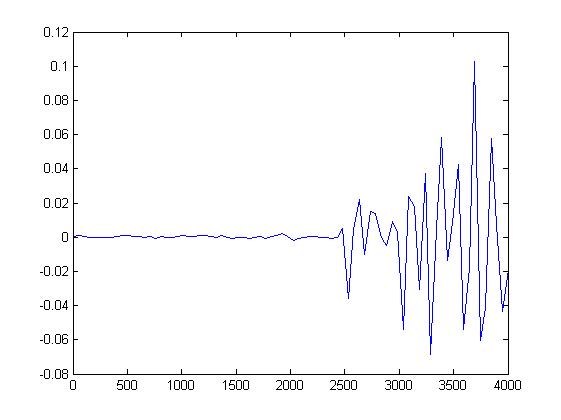
\includegraphics[width=0.7\textwidth]{signal.jpg}}
		\subfigure[][Spectrum (blue) and extracted features (red)]{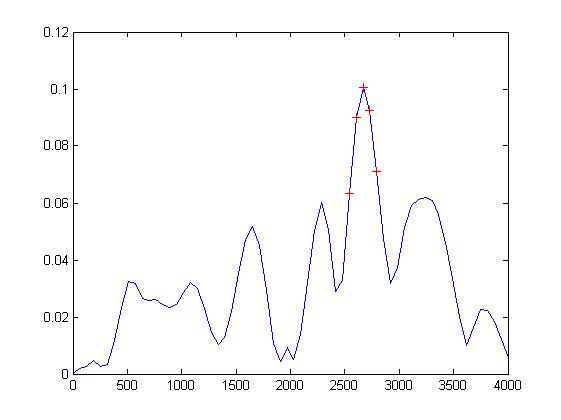
\includegraphics[width=0.7\textwidth]{spectrum.jpg}}
	\label{fig:frame}
	\caption{Frame 2 of file \lstinline&stop_1.wav&}
\end{figure}

\section{Recognition Framework}\label{sec:hmm}
Part two of the project was the building of the basic recognition system except of filling it with wise values for the different models (for that see section \ref{sec:learn}). The recognition system is basically encapsulated in the class \lstinline&classifier&, like already discussed in section \ref{sec:system}. The core of the recognition lays in the HMMs which are realised in a class \lstinline&hmm&. In the design we followed the suggestion from the project notes as well as we took over the \lstinline&forwardHMM& function with just one or two adjustments, for example, the return of matrix \textbf{B} (used for learning). In there a \lstinline&calcLikelihood& called function is used to calculate the likelihood of the observed data. This function applies a multivariate normal (Gaussian) distribution (no mixture of several distributions) to every feature entry. That means we get one likelihood for each feature. These likelihoods are added up weighted, so that the likelihood of the greatest magnitude in the spectrum influences most.


\section{Learning}

\begin{lstlisting}
\end{lstlisting}

\end{document}
 
